\documentclass[aspectratio=169, table, 12pt]{beamer}

\usepackage{colortbl}
\usepackage{xcolor}
\usepackage{listings}
\usepackage{tabularx}
\usepackage{tikz}
\usetikzlibrary{arrows.meta, positioning, calc, fit,
  shapes.geometric, backgrounds}

\makeatletter
\def\input@path{{../theme/}}
\makeatother
\graphicspath{{../theme/}{../../figures/}}
\usetheme{Pradita}

\definecolor{praditagreen}{RGB}{37, 113, 71}

% Tema membuat garis tabel berwarna putih. Dikembalikan agar tabel terbaca.
\arrayrulecolor{black}
\setlength{\arrayrulewidth}{0.5pt}

\lstdefinestyle{PythonStyle}{
  language=Python,
  basicstyle=\ttfamily\scriptsize,
  keywordstyle=\color{blue}\bfseries,
  commentstyle=\color{gray}\itshape,
  stringstyle=\color{red},
  breaklines=true,
  frame=lines,
  backgroundcolor=\color{lightgray!10},
  tabsize=2,
  showstringspaces=false
}

\lstdefinelanguage{bash}{
  keywords={},
  basicstyle=\ttfamily\scriptsize,
  ndkeywords={cd, python, bash, source},
  ndkeywordstyle=\color{purple}\bfseries,
  sensitive=true,
  commentstyle=\color{gray},
  breaklines=true,
  frame=lines,
  backgroundcolor=\color{lightgray!10},
  tabsize=2,
  comment=[l]{\#},
  showstringspaces=false
}

\title{\Huge{Event-Driven Architecture}}
\subtitle{IF231303 Arsitektur Perangkat Lunak}
\author{Alfa Yohannis}

\begin{document}

\frame{\titlepage}

\begin{frame}{{\Large Tujuan Pembelajaran}}
  \vspace{10pt}
  \begin{enumerate}
    \item Menjelaskan pembagian antara penerbit, event, dan pelanggan beserta
          kontrak yang menghubungkan ketiganya.
    \item Membedakan topologi broker dari topologi mediator, lalu menentukan
          kapan masing-masing layak dipilih.
    \item Mengukur \textit{latency cost}, \textit{failure containment}, dan
          \textit{change cost} pada ketiga susunan.
  \end{enumerate}

  \vspace{10pt}
  {\small Contohnya satu permintaan konversi kurs, dibuat tiga susunan yang
  memanggil pemroses yang sama persis.}
\end{frame}

\begin{frame}{{\Large Pendahuluan}}
  \vspace{8pt}
  \begin{itemize}\small
    \item Satu permintaan konversi kurs perlu dicatat ke riwayat, diperiksa
          nilainya, lalu diberitahukan kepada pemohon.
    \item Cara paling lurus memanggil ketiga pekerjaan itu berurutan dari satu
          tempat, sehingga pemanggilnya terikat pada ketiganya sekaligus.
    \item \textit{Event-driven architecture} melonggarkan ikatan itu, yaitu
          pemanggil cukup mengumumkan bahwa sesuatu telah terjadi lalu berhenti.
    \item Pihak yang berkepentingan mendaftarkan diri sendiri, dan pengumuman
          itu sampai kepada mereka tanpa disebut namanya.
  \end{itemize}

  \vspace{8pt}
  {\small Kedua topologi berbasis event pada bab ini mengikuti kerangka Richards
  dan Ford, sedangkan nama pola \textit{message}-nya mengikuti katalog Hohpe dan Woolf.}
\end{frame}

\begin{frame}{{\Large Istilah yang Dipakai}}
  \vspace{10pt}
  \begin{itemize}\small
    \item \textbf{Penerbit} mengumumkan bahwa sesuatu telah terjadi, lalu
          selesai tanpa menunggu siapa pun.
    \item \textbf{Event} adalah \textit{message} yang membawa kabar tersebut beserta
          datanya.
    \item \textbf{Pelanggan} menyatakan minat pada satu jenis kabar, lalu
          mengerjakan bagiannya setiap kali kabar itu datang.
    \item \textbf{Topik} adalah nama saluran tempat kabar diumumkan, dan setiap
          pelanggan topik tersebut punya antrean sendiri.
  \end{itemize}

  \vspace{10pt}
  {\small Saluran seperti itu disebut \textit{publish-subscribe channel}, sebab
  satu salinan dikirim kepada setiap pelanggan.}
\end{frame}

\begin{frame}{{\Large Event, Bukan Perintah}}
  \vspace{10pt}
  \begin{itemize}\small
    \item Nama \texttt{permintaan.dicatat} menyebut sesuatu yang sudah terjadi,
          sehingga penerbitnya tidak menuntut apa pun.
    \item Nama \texttt{catat\_permintaan} menyebut sesuatu yang harus
          dikerjakan, sehingga penerbitnya menuntut satu pekerjaan tertentu.
    \item Nama kedua memaksa penerbit tahu bahwa ada pihak yang mencatat, dan
          ikatan itulah yang sebenarnya hendak dilepas.
    \item Penamaan karena itu bukan soal selera, melainkan penentu siapa
          mengenal siapa.
  \end{itemize}

  \vspace{10pt}
  {\small Seluruh topik pada bab ini memakai bentuk pertama, yaitu
  \texttt{permintaan.diterima}, \texttt{permintaan.dicatat}, dan
  \texttt{permintaan.diperiksa}.}
\end{frame}

\begin{frame}{{\Large Alur Penerbit ke Pelanggan}}
  \vspace{4pt}
  \begin{center}
    \resizebox{0.86\textwidth}{!}{%
      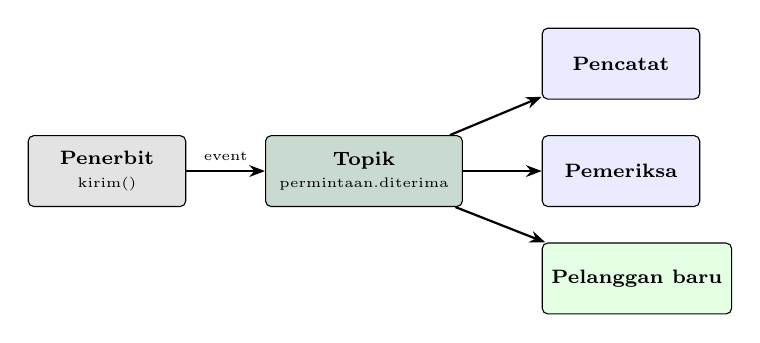
\begin{tikzpicture}[
        kotak/.style={draw, rounded corners=2pt, minimum width=2.0cm,
          minimum height=0.9cm, align=center, font=\scriptsize\bfseries},
        panah/.style={-{Stealth[length=2mm]}, thick}
      ]
        \node[kotak, fill=gray!22] (penerbit) {Penerbit\\
          {\tiny\mdseries kirim()}};
        \node[kotak, fill=praditagreen!25, right=1.0cm of penerbit,
          minimum width=2.5cm] (topik) {Topik\\
          {\tiny\mdseries permintaan.diterima}};
        \node[kotak, fill=blue!8, above right=0.45cm and 1.0cm of topik] (p1)
          {Pencatat};
        \node[kotak, fill=blue!8, right=1.0cm of topik] (p2) {Pemeriksa};
        \node[kotak, fill=green!10, below right=0.45cm and 1.0cm of topik] (p3)
          {Pelanggan baru};

        \draw[panah] (penerbit) -- node[above, font=\tiny] {event} (topik);
        \draw[panah] (topik) -- (p1);
        \draw[panah] (topik) -- (p2);
        \draw[panah] (topik) -- (p3);
      \end{tikzpicture}}
  \end{center}

  \vspace{4pt}
  {\small Penerbit hanya mengenal nama topik. Pelanggan mendaftarkan dirinya
  sendiri, sehingga kotak baru di sisi kanan dapat muncul tanpa menyentuh kotak
  di sisi kiri.}
\end{frame}

\begin{frame}{{\Large Pembagian Ketiga Peran}}
  \vspace{6pt}
  {\small Pembagian ini menentukan letak setiap keputusan, termasuk apa yang
  sengaja tidak boleh diketahui.}

  \vspace{6pt}
  \centering
  \small
  \begin{tabularx}{0.96\textwidth}{|l|X|X|}
    \hline
    \textbf{Peran} & \textbf{Tanggung jawab} & \textbf{Tidak boleh mengetahui} \\
    \hline
    Penerbit & Mengumumkan kabar beserta datanya pada satu topik & Nama, jumlah, dan nasib pelanggan mana pun \\
    \hline
    Event & Membawa kabar yang sudah terjadi, bukan perintah & Cara pelanggan mengerjakan bagiannya \\
    \hline
    Pelanggan & Mengerjakan satu bagian setiap kali kabarnya datang & Nama pelanggan lain pada topik yang sama \\
    \hline
  \end{tabularx}
\end{frame}

\begin{frame}{{\Large Analogi: Pengeras Suara Kampus}}
  \vspace{10pt}
  \begin{itemize}\small
    \item Petugas membacakan bahwa jadwal ujian sudah terbit, lalu meletakkan
          mikrofonnya.
    \item Petugas itu tidak menghubungi mahasiswa satu per satu, dan tidak
          menunggu satu pun tanggapan.
    \item Mahasiswa yang berkepentingan mendengar lalu mengerjakan urusannya
          masing-masing, sedangkan yang berada di luar gedung tidak mendengar
          apa pun.
    \item Pengumuman yang sudah dibacakan juga tidak dapat ditarik kembali.
  \end{itemize}

  \vspace{10pt}
  {\small Ketiga sifat itulah yang dibawa event, yaitu penerbit tidak mengenal
  penerima, penerima dapat melewatkannya, dan kabarnya tidak dapat dibatalkan.}
\end{frame}

\begin{frame}{{\Large Topologi Broker}}
  \vspace{14pt}
  \begin{columns}[c]
    \begin{column}{0.40\textwidth}
      \centering
      \resizebox{!}{0.52\textheight}{%
        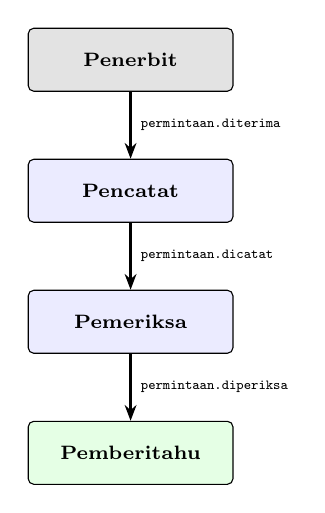
\begin{tikzpicture}[
          kotak/.style={draw, rounded corners=2pt, minimum width=2.6cm,
            minimum height=0.8cm, align=center, font=\scriptsize\bfseries},
          panah/.style={-{Stealth[length=2mm]}, thick}
        ]
          \node[kotak, fill=gray!22] (penerbit) {Penerbit};
          \node[kotak, fill=blue!8, below=0.85cm of penerbit] (catat)
            {Pencatat};
          \node[kotak, fill=blue!8, below=0.85cm of catat] (periksa)
            {Pemeriksa};
          \node[kotak, fill=green!10, below=0.85cm of periksa] (beritahu)
            {Pemberitahu};

          \draw[panah] (penerbit) -- node[right, font=\tiny]
            {\texttt{permintaan.diterima}} (catat);
          \draw[panah] (catat) -- node[right, font=\tiny]
            {\texttt{permintaan.dicatat}} (periksa);
          \draw[panah] (periksa) -- node[right, font=\tiny]
            {\texttt{permintaan.diperiksa}} (beritahu);
        \end{tikzpicture}}
    \end{column}
    \begin{column}{0.56\textwidth}
      \begin{itemize}\small
        \item Tidak ada yang memegang urutan langkahnya.
        \item Setiap pelanggan bekerja, lalu menerbitkan event tentang
              pekerjaannya sendiri.
        \item Pelanggan berikutnya mendengar event itu, lalu menerbitkan event
              berikutnya lagi.
        \item Urutan langkah karena itu tersebar pada pilihan topik setiap
              pelanggan.
      \end{itemize}
    \end{column}
  \end{columns}
\end{frame}

\begin{frame}[fragile]{{\Large Kode: Inti Broker}}
  \vspace{2pt}
\begin{lstlisting}[style=PythonStyle]
def terbitkan(self, topik: str, pesan: domain.Permintaan) -> int:
  """Menaruh pesan pada antrean setiap pelanggan topik tersebut."""
  antrean_pelanggan = self.langganan_topik.get(topik, [])
  for antrean in antrean_pelanggan:
    antrean.put(pesan)
  with self.kunci:
    self.jumlah_pesan += len(antrean_pelanggan)
  return len(antrean_pelanggan)

def saat_diterima(self, permintaan: domain.Permintaan) -> None:
  """Mencatat permintaan, lalu mengumumkan bahwa pencatatannya selesai."""
  self.pencatat.tangani(permintaan)
  self.broker.terbitkan(TOPIK_DICATAT, permintaan)
\end{lstlisting}

  \vspace{2pt}
  {\small Brokernya kecil, sebab yang disimpannya hanya nama topik beserta
  daftar antreannya. Rantainya sependek satu panggilan lalu satu penerbitan.}
\end{frame}

\begin{frame}{{\Large Topologi Mediator}}
  \vspace{2pt}
  \begin{center}
    \hspace*{-1.4cm}\resizebox{0.62\textwidth}{!}{%
      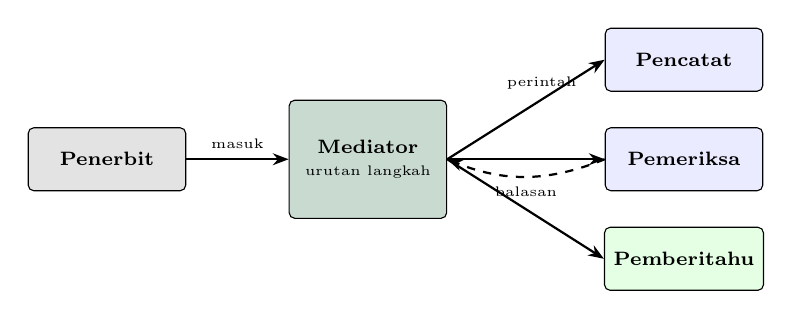
\begin{tikzpicture}[
        kotak/.style={draw, rounded corners=2pt, minimum width=2.0cm,
          minimum height=0.8cm, align=center, font=\scriptsize\bfseries},
        panah/.style={-{Stealth[length=2mm]}, thick},
        balasan/.style={-{Stealth[length=2mm]}, thick, dashed}
      ]
        \node[kotak, fill=gray!22] (penerbit) {Penerbit};
        \node[kotak, fill=praditagreen!25, right=1.3cm of penerbit,
          minimum height=1.5cm] (mediator) {Mediator\\
          {\tiny\mdseries urutan langkah}};
        \node[kotak, fill=blue!8, right=2.0cm of mediator] (periksa)
          {Pemeriksa};
        \node[kotak, fill=blue!8, above=0.45cm of periksa] (catat) {Pencatat};
        \node[kotak, fill=green!10, below=0.45cm of periksa] (beritahu)
          {Pemberitahu};

        \draw[panah] (penerbit) -- node[above, font=\tiny] {masuk} (mediator);
        \draw[panah] (mediator.east) -- node[above, font=\tiny, pos=0.6]
          {perintah} (catat.west);
        \draw[panah] (mediator.east) -- (periksa.west);
        \draw[panah] (mediator.east) -- (beritahu.west);
        \draw[balasan] (periksa.west) to[bend left=22]
          node[below, font=\tiny, pos=0.5] {balasan} (mediator.east);
      \end{tikzpicture}}
  \end{center}

  \vspace{2pt}
  \begin{itemize}\small
    \item Penerbit mengirim permintaan ke satu pengatur, dan pengatur itulah
          yang memegang daftar langkahnya.
    \item Pengatur memanggil pemroses pertama, menunggu balasannya, lalu
          memanggil pemroses kedua.
    \item Karena menunggu, pengatur tahu langkah mana yang gagal dan langkah
          mana yang belum dijalankan.
  \end{itemize}
\end{frame}

\begin{frame}[fragile]{{\Large Kode: Urutan Langkah Mediator}}
  \vspace{2pt}
\begin{lstlisting}[style=PythonStyle]
def jalankan_urutan(self, permintaan: domain.Permintaan) -> bool:
  """Memanggil setiap pemroses bergantian, lalu berhenti pada galat pertama."""
  for nomor_langkah, nama in enumerate(self.urutan):
    self.antrean_perintah[nama].put(permintaan)
    self.hitung_pesan(1)
    _, _, galat = self.antrean_balasan.get()
    if galat is not None:
      sisa = self.urutan[nomor_langkah + 1:]
      self.gagal.append((permintaan.nomor, nama, list(sisa)))
      return False
  return True
\end{lstlisting}

  \vspace{2pt}
  {\small Isi pengaturnya hanya satu perulangan. Ketika satu langkah gagal, yang
  dicatat bukan hanya nama langkahnya, melainkan juga sisa langkah yang belum
  dijalankan.}
\end{frame}

\begin{frame}{{\Large Analogi: Ketua Panitia Wisuda}}
  \vspace{10pt}
  \begin{itemize}\small
    \item Ketua memegang susunan acara, menelepon seksi konsumsi, menunggu
          laporan selesai, baru menelepon seksi dekorasi.
    \item Bila seksi konsumsi melapor gagal, ketua tahu acara berhenti di \textit{identifier}
          itu dan tahu seksi mana yang belum dihubungi.
    \item Harganya, setiap kabar melewati satu orang yang sama, dan orang itu
          hanya dapat menangani satu urusan pada satu waktu.
  \end{itemize}

  \vspace{10pt}
  {\small Kedua akibat itu muncul kembali sebagai angka, yaitu catatan langkah
  yang putus pada seksi ketahanan dan waktu tunggu pada seksi berikutnya.}
\end{frame}

\begin{frame}{{\Large \textit{Class Diagram}: Broker dan Mediator}}
  \vspace{4pt}
  \begin{center}
    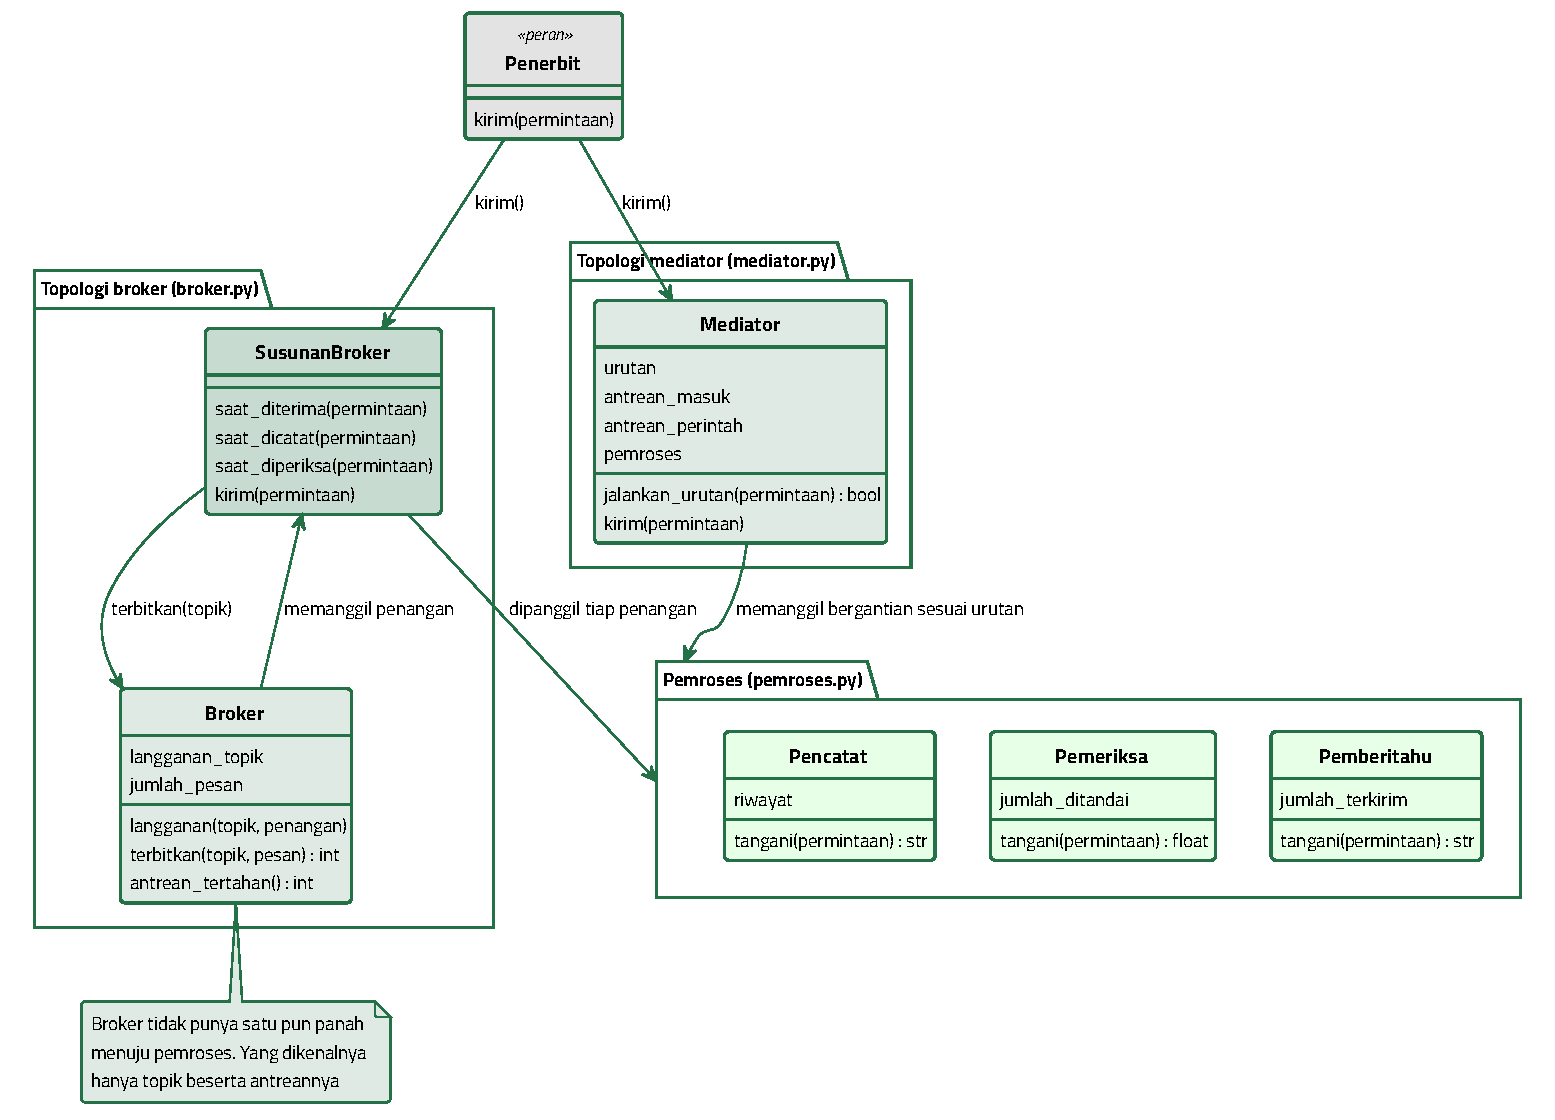
\includegraphics[width=\textwidth, height=0.74\textheight,
      keepaspectratio]{kelas-event.pdf}
  \end{center}
\end{frame}

\begin{frame}{{\Large Penjelasan \textit{Class Diagram}}}
  \vspace{10pt}
  \begin{itemize}\small
    \item Perbedaan pokok kedua topologi terbaca dari arah panahnya, bukan dari
          jumlah kelasnya.
    \item Tidak ada satu pun panah dari \texttt{Broker} menuju pemroses. Yang
          dikenalnya hanya topik beserta antreannya.
    \item \texttt{Mediator} justru menyimpan rujukan ke setiap pemroses, sebab
          urutan langkah memang dipegangnya.
    \item Ketiga pemroses sama persis pada kedua topologi, sehingga selisih
          waktunya nanti hanya berasal dari cara \textit{message}-nya disampaikan.
  \end{itemize}
\end{frame}

\begin{frame}{{\Large \textit{Sequence Diagram}: Satu Permintaan}}
  \vspace{4pt}
  \begin{center}
    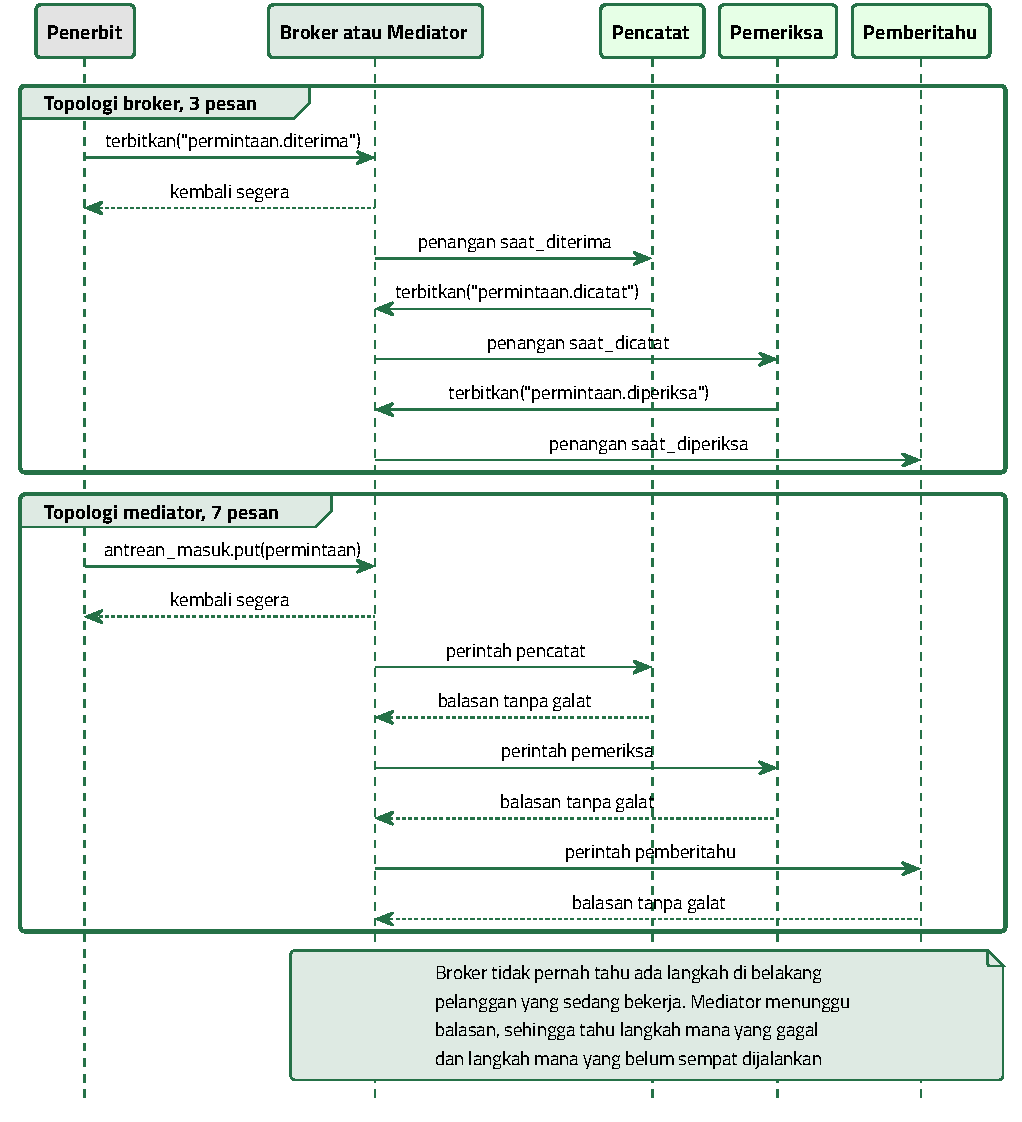
\includegraphics[width=0.92\textwidth, height=0.74\textheight,
      keepaspectratio]{sekuens-event.pdf}
  \end{center}
\end{frame}

\begin{frame}{{\Large Penjelasan \textit{Sequence Diagram}}}
  \vspace{10pt}
  \begin{itemize}\small
    \item Pekerjaan domainnya sama pada kedua topologi, yang berbeda jumlah
          \textit{message} yang mengangkutnya.
    \item Pada topologi broker, satu permintaan menempuh tiga \textit{message}, yaitu satu
          event per langkah.
    \item Pada topologi mediator, permintaan yang sama menempuh tujuh \textit{message},
          sebab setiap langkah berupa satu perintah beserta satu balasan.
    \item Balasan itulah yang dibeli, yaitu mediator tahu langkah mana yang
          gagal sedangkan broker tidak pernah tahu ada langkah di belakangnya.
  \end{itemize}
\end{frame}

\begin{frame}{{\Large Jumlah \textit{Message} per Permintaan}}
  \vspace{6pt}
  {\small Angkanya dihitung skrip, bukan ditaksir, dan menjadi dasar
  perbandingan seluruh seksi hasil.}

  \vspace{6pt}
  \centering
  \small
  \begin{tabularx}{0.96\textwidth}{|l|l|X|}
    \hline
    \textbf{Susunan} & \textbf{\textit{Message}} & \textbf{Rinciannya} \\
    \hline
    Sinkron & 0 & Ketiga langkah berupa pemanggilan langsung di dalam satu \textit{thread} \\
    \hline
    Broker & 3 & Satu event per langkah, masing-masing menuju satu pelanggan \\
    \hline
    Mediator & 7 & Satu \textit{message} masuk, ditambah satu perintah dan satu balasan per langkah \\
    \hline
  \end{tabularx}

  \vspace{6pt}
  \raggedright
  {\small Susunan sinkron adalah pembandingnya, yaitu panggilan berantai
  langsung tanpa antrean sama sekali.}
\end{frame}

\begin{frame}{{\Large Hasil: \textit{Latency Cost}}}
  \vspace{6pt}
  {\small Dua ratus permintaan, ketiga susunan diukur berselang-seling di dalam
  putaran yang sama. Satuannya milidetik.}

  \vspace{6pt}
  \centering
  \small
  \begin{tabularx}{0.96\textwidth}{|l|l|l|l|l|X|}
    \hline
    \textbf{Susunan} & \textbf{Median} & \textbf{P95} & \textbf{Terbesar} & \textbf{Kembali} & \textbf{\textit{Message}} \\
    \hline
    Sinkron & 0,0065 & 0,0108 & 0,0230 & 0,0059 & 0 \\
    \hline
    Broker & 0,0361 & 0,0600 & 0,0730 & 0,0029 & 3 \\
    \hline
    Mediator & 0,0544 & 0,0725 & 0,1129 & 0,0025 & 7 \\
    \hline
  \end{tabularx}

  \vspace{6pt}
  \raggedright
  {\small Kolom median sampai terbesar dihitung sampai langkah terakhir selesai,
  sedangkan kolom kembali dihitung sampai fungsi \texttt{kirim} kembali.}
\end{frame}

\begin{frame}{{\Large Membaca Hasilnya}}
  \vspace{10pt}
  \begin{itemize}\small
    \item Angka itu menolak harapan yang sering dibawa ke bab ini, yaitu bahwa
          event membuat permintaan lebih cepat.
    \item Median topologi broker 5,5 kali median susunan sinkron, dan topologi
          mediator 8,3 kali.
    \item \textit{Range} jalur sinkron 0,0177 ms, sedangkan selisih median
          terhadap broker 0,0296 ms, yaitu 1,7 kali \textit{range} itu.
    \item Susunan sinkron lebih cepat pada 200 dari 200 putaran, sehingga
          selisihnya bukan kebetulan.
  \end{itemize}

  \vspace{10pt}
  {\small Sebabnya perpindahan antar \textit{thread}. Pekerjaan pada bab ini
  hanya satu perkalian dan dua penyusunan teks, sehingga \textit{cost}
  pengangkutannya justru mendominasi.}
\end{frame}

\begin{frame}{{\Large Kejanggalan Kolom Kembali}}
  \vspace{10pt}
  \begin{itemize}\small
    \item Susunan broker kembali 0,0030 ms lebih cepat daripada susunan sinkron,
          yaitu 0,0029 ms berbanding 0,0059 ms.
    \item \textit{Range} jalur sinkron 5,9 kali lebih besar daripada selisih
          itu, sehingga menurut ukuran Bab 2 selisihnya belum dapat disebut ada.
    \item Pencacahan per putaran justru menunjuk arah yang jelas, yaitu susunan
          berbasis event kembali lebih cepat pada 199 dari 200 putaran.
    \item Pencacahan lebih peka daripada median, sebab median menyerap satu
          putaran lambat sebagai angka besar sedangkan pencacahan hanya melihat
          siapa yang menang.
  \end{itemize}

  \vspace{10pt}
  {\small Selisih sekecil itu memang belum menarik. Yang menarik apa yang
  terjadi padanya ketika satu pemroses mulai lambat.}
\end{frame}

\begin{frame}{{\Large Kasus: Loket Pembayaran}}
  \vspace{10pt}
  \begin{itemize}\small
    \item Loket memakai susunan sinkron, yaitu setiap pembayaran dicatat,
          diperiksa, lalu diberitahukan lewat layanan \textit{message} singkat pihak
          ketiga.
    \item Pada hari biasa layanan itu menjawab dalam puluhan milidetik.
    \item Pada hari terakhir pembayaran, layanan tersebut tersendat dan
          jawabannya berubah menjadi lima detik.
    \item Petugas tidak dapat menerima pembayaran berikutnya sebelum jawaban itu
          datang, antrean mahasiswa mengular, dan sebagian pulang tanpa
          membayar.
  \end{itemize}

  \vspace{10pt}
  {\small Pencatatan dan pemeriksaannya sendiri sebenarnya sudah selesai sejak
  awal, sehingga yang menahan loket adalah langkah terakhirnya.}
\end{frame}

\begin{frame}{{\Large Hasil: \textit{Failure Containment}}}
  \vspace{6pt}
  {\small Seratus permintaan, pemeriksanya menolak setiap permintaan kelipatan
  lima.}

  \vspace{6pt}
  \centering
  \small
  \begin{tabularx}{0.96\textwidth}{|l|l|l|l|l|X|}
    \hline
    \textbf{Susunan} & \textbf{Tuntas} & \textbf{Tercatat} & \textbf{Diberitahu} & \textbf{Galat} & \textbf{Berhenti} \\
    \hline
    Sinkron & 4 & 5 & 4 & 0 & pada nomor 5 \\
    \hline
    Broker & 80 & 100 & 80 & 20 & tidak \\
    \hline
    Mediator & 80 & 100 & 80 & 20 & tidak \\
    \hline
  \end{tabularx}

  \vspace{6pt}
  \raggedright
  {\small Susunan sinkron berhenti pada permintaan kelima, sehingga sembilan
  puluh lima permintaan sesudahnya tidak pernah tersentuh. Kedua susunan
  berbasis event menampung galatnya di dalam \textit{thread} pelanggan.}
\end{frame}

\begin{frame}{{\Large Catatan Galat Kedua Topologi}}
  \vspace{10pt}
  \begin{itemize}\small
    \item Angka keduanya sama, yaitu 80 tuntas dan 100 tercatat, namun catatan
          galatnya berbeda.
    \item Broker mencatat topik beserta nomor permintaannya, yaitu
          \texttt{topik permintaan.dicatat, permintaan 5}.
    \item Mediator mencatat langkah yang gagal sekaligus sisanya, yaitu
          \texttt{permintaan 5 putus pada pemeriksa, sisa ['pemberitahu']}.
    \item Hanya mediator yang memegang urutan lengkapnya, sehingga hanya
          mediator yang dapat mengulang sisa langkah itu kelak.
  \end{itemize}

  \vspace{10pt}
  {\small Itulah yang dibeli dengan empat \textit{message} tambahan per permintaan.}
\end{frame}

\begin{frame}{{\Large Hasil: Penerbit Tertahan}}
  \vspace{6pt}
  {\small Seratus permintaan, pemeriksanya menahan lima milidetik. Seluruh
  waktunya untuk seratus permintaan sekaligus, bukan per permintaan.}

  \vspace{6pt}
  \centering
  \footnotesize
  \begin{tabularx}{0.96\textwidth}{|l|l|l|l|>{\raggedright\arraybackslash}X|}
    \hline
    \textbf{Susunan} & \textbf{Penerbit kembali} & \textbf{Antrean terdalam} & \textbf{Seluruh tercatat} & \textbf{Seluruh tuntas} \\
    \hline
    Sinkron & 517,6 ms & 0 & 518,0 ms & 518,2 ms \\
    \hline
    Broker & 0,4 ms & 100 & 1,9 ms & 518,4 ms \\
    \hline
    Mediator & 0,4 ms & 100 & 543,7 ms & 548,2 ms \\
    \hline
  \end{tabularx}

  \vspace{6pt}
  \raggedright
  {\small Antrean terdalam adalah jumlah \textit{message} terbanyak yang pernah menumpuk
  pada satu antrean selama percobaan berjalan.}
\end{frame}

\begin{frame}{{\Large Membaca Hasilnya}}
  \vspace{10pt}
  \begin{itemize}\small
    \item Penerbit sinkron tertahan 517,6 ms, sedangkan penerbit pada kedua
          susunan berbasis event kembali sesudah 0,4 ms. Perbandingannya lebih
          dari seribu kali.
    \item Pekerjaan yang tidak lagi ditunggu penerbit tidak lenyap, melainkan
          menumpuk, dan puncaknya seratus \textit{message}.
    \item Seratus permintaan selesai dicatat sesudah 1,9 ms pada topologi
          broker, sedangkan topologi mediator membutuhkan 543,7 ms.
    \item Sebabnya, pencatat broker punya antrean sendiri dan tidak menunggu
          pemeriksa, sedangkan mediator menangani satu permintaan pada satu
          waktu.
  \end{itemize}

  \vspace{10pt}
  {\small Pengawasan terpusat karena itu bukan hanya menambah \textit{message}, melainkan
  juga membuat pengaturnya menjadi leher botol.}
\end{frame}

\begin{frame}{{\Large Hasil: \textit{Change Cost}}}
  \vspace{6pt}
  {\small Bagian audit meminta setiap permintaan disalin ke jurnal tersendiri,
  sehingga satu pemroses baru disisipkan pada ketiga susunan.}

  \vspace{6pt}
  \centering
  \small
  \begin{tabularx}{0.96\textwidth}{|l|l|l|l|X|}
    \hline
    \textbf{Susunan} & \textbf{Baris tambah} & \textbf{Baris hapus} & \textbf{\textit{Message} sebelum} & \textbf{\textit{Message} sesudah} \\
    \hline
    Sinkron & 6 & 3 & 0 & 0 \\
    \hline
    Broker & 3 & 0 & 3 & 4 \\
    \hline
    Mediator & 3 & 1 & 7 & 9 \\
    \hline
  \end{tabularx}

  \vspace{6pt}
  \raggedright
  {\small Selisih barisnya kecil, dan kekecilan itu jujur. Yang lebih
  menentukan letak barisnya, yaitu badan \texttt{kirim} pada susunan sinkron
  dan bagian perakitan pada kedua topologi berbasis event.}
\end{frame}

\begin{frame}{{\Large Urutan Antar Pelanggan}}
  \vspace{10pt}
  \begin{itemize}\small
    \item Pada topologi mediator, jejak langkahnya selalu \texttt{pencatat,
          pemeriksa, pemberitahu, audit}.
    \item Pada topologi broker, dua belas kali penjalanan menghasilkan tiga
          bentuk, yaitu \texttt{audit} di urutan pertama delapan kali, terakhir
          tiga kali, dan kedua satu kali.
    \item Sebabnya, pencatat audit berlangganan pada topik yang sama dengan
          pencatat biasa, sehingga keduanya berjalan sejajar di \textit{thread}
          masing-masing.
    \item Akibatnya, urutan antar pelanggan satu topik tidak boleh diandalkan.
  \end{itemize}

  \vspace{10pt}
  {\small Pelanggan baru juga menambah satu \textit{message} per permintaan pada broker dan
  dua \textit{message} pada mediator.}
\end{frame}

\begin{frame}{{\Large \textit{Summary}}}
  \vspace{10pt}
  \begin{itemize}\small
    \item Penerbit mengumumkan bahwa sesuatu telah terjadi lalu berhenti, dan
          pelanggan mendaftarkan dirinya sendiri pada topik yang diminatinya.
    \item Kelonggaran itu dibayar dengan waktu, yaitu latensi broker 5,5 kali
          latensi sinkron dan mediator 8,3 kali, sedangkan sinkron menang pada
          200 dari 200 putaran.
    \item Yang dibeli terlihat saat satu pemroses tersendat, yaitu penerbit
          sinkron tertahan 517,6 ms sedangkan penerbit berbasis event kembali
          sesudah 0,4 ms.
    \item Broker memakai tiga \textit{message} dan melepas langkah pertama dari langkah
          lambat di belakangnya, sedangkan mediator memakai tujuh \textit{message} namun
          tahu langkah mana yang putus beserta sisanya.
  \end{itemize}

  \vspace{10pt}
  {\small \textit{Message} utamanya, event memindahkan waktu tunggu dari penerbit ke
  antrean, dan tumpukan seratus \textit{message} itulah yang harus dipantau.}
\end{frame}

\begin{frame}[fragile]{{\Large Persiapan Latihan}}
  \vspace{5pt}
\begin{lstlisting}[language=bash]
bash sources/siapkan_venv.sh
source .venv/bin/activate
cd sources/chapter09
python sinkron.py
# Pesan lewat antrean: 0
python broker.py
# Pesan lewat antrean: 3
python mediator.py
# Pesan lewat antrean: 7
\end{lstlisting}

  \vspace{6pt}
  {\small Bab ini hanya memakai pustaka standar Python. Langkah lengkap, tabel
  contoh, dan lembar isian ada di modul Bab 9, yang menjadi rujukan utama
  latihan ini.}
\end{frame}

\begin{frame}[fragile]{{\Large Latihan 1: \textit{Latency Cost}}}
  \vspace{2pt}
  {\small Tujuan: menguji harapan bahwa event membuat satu permintaan lebih
  cepat.}

  \vspace{2pt}
\begin{lstlisting}[language=bash]
python ukur_latensi.py
# sinkron   0.0065 ms  p95 0.0108  terbesar 0.0230  pesan 0
# mediator  0.0544 ms  p95 0.0725  terbesar 0.1129  pesan 7
# putaran sinkron lebih cepat  : 200 dari 200
\end{lstlisting}

  \vspace{2pt}
  \begin{enumerate}\small
    \item Catat keenam angka pada baris ringkasan ketiga susunan.
    \item Catat \textit{range} jalur sinkron, selisih median, dan pencacahan
          putarannya.
    \item Buka \texttt{mediator.py}, lalu hitung sendiri asal angka tujuh \textit{message}.
    \item Ubah \texttt{JUMLAH\_PERMINTAAN} menjadi lima ratus, lalu catat
          perubahan persentil ke-95 dan nilai terbesarnya.
  \end{enumerate}

  \vspace{2pt}
  {\small Pertanyaan: mengapa susunan sinkron justru paling cepat?}
\end{frame}

\begin{frame}[fragile]{{\Large Latihan 2: \textit{Failure Containment}}}
  \vspace{2pt}
  {\small Tujuan: membuktikan satu pemroses yang gagal tidak menjatuhkan
  seluruhnya.}

  \vspace{2pt}
\begin{lstlisting}[language=bash]
python uji_ketahanan.py
# sinkron   tuntas   4  tercatat   5  berhenti pada 5
# broker    tuntas  80  tercatat 100  berhenti tidak
# sinkron   penerbit kembali 517.6 ms  antrean   0
# broker    penerbit kembali   0.4 ms  antrean 100
\end{lstlisting}

  \vspace{2pt}
  \begin{enumerate}\small
    \item Tunjukkan baris pada \texttt{pemroses.py} yang membuat
          \texttt{PemeriksaGagal} menolak.
    \item Catat kedua tabel hasilnya beserta ketiga contoh catatan
          \textit{error}-nya.
    \item Naikkan \texttt{JEDA\_LAMBAT} menjadi lima puluh milidetik, lalu catat
          perubahan antrean terdalam dan waktu penerbit kembali.
  \end{enumerate}

  \vspace{2pt}
  {\small Pertanyaan: apa yang diketahui mediator dan tidak diketahui broker?}
\end{frame}

\begin{frame}[fragile]{{\Large Latihan 3: \textit{Change Cost}}}
  \vspace{2pt}
  {\small Tujuan: menghitung biaya menyisipkan satu pelanggan baru.}

  \vspace{2pt}
\begin{lstlisting}[language=bash]
python ukur_perubahan.py
# sinkron   tambah 6  hapus 3  pesan 0.0 lalu 0.0
# broker    tambah 3  hapus 0  pesan 3.0 lalu 4.0
# Jejak broker: ['audit', 'pencatat', 'pemeriksa', 'pemberitahu']
\end{lstlisting}

  \vspace{2pt}
  \begin{enumerate}\small
    \item Catat ketiga baris tabelnya beserta ketiga jejak langkahnya.
    \item Bandingkan \texttt{broker.py} dengan versi di
          \texttt{varian\_audit/}, lalu tunjukkan baris yang berbeda.
    \item Sisipkan sendiri audit pada \texttt{sinkron.py}, lalu catat baris
          alur bisnis yang tersentuh.
    \item Jalankan ulang beberapa kali, lalu catat apakah jejak broker selalu
          sama.
  \end{enumerate}

  \vspace{2pt}
  {\small Pertanyaan: kapan topologi broker lebih tepat daripada mediator?}
\end{frame}

\end{document}
